% !TEX TS-program = Xelatex
% !TEX encoding = UTF-8 Unicode

\documentclass[UTF8]{ctexart}
\usepackage{amsmath}
\usepackage[bottom]{footmisc}
\usepackage{geometry}
\usepackage{hyperref}
\usepackage{graphicx}
\usepackage{figsize}
\usepackage[separate-uncertainty = true,per-mode=symbol]{siunitx}
\usepackage{tabu}
\usepackage{wasysym}
\geometry{left=0.7in,right=0.7in,bottom=0.7in,top=0.7in}

\title{实验十:气垫导轨上的弹簧振子}
\author{朱寅杰 1600017721}
\date{2017年12月15日}

\begin{document}
\maketitle
\paragraph{研究弹簧振子周期与振幅的关系}
在气垫导轨上设置一个弹簧振子,从标尺上读出其平衡位置在$x_0=\SI{100.3}{\cm}$。分别将弹簧振子从平衡位置左右不同距离处释放,使用放在平衡位置的光电门计数器测量振子的周期。实验时分别在平衡位置左右距离为\SI{10}{\cm}、\SI{20}{\cm}、\SI{30}{\cm}和\SI{40}{\cm}处静止释放,每个位置都测量三次以确认测量的精确程度。每次测量记录到的周期(单位:秒),以及它们的平均值和平均值的不确定度列于下表中:
\begin{center}
\begin{tabu} to \linewidth {X[c]|X[c]X[c]X[c]|X[c]X[c]X[c]|X[c]X[c]}
\hline
$A$/\si{\cm}	&左1	&2	&3	&右1	&右2	&右3	&$\bar{T}/\si{s}$&$\sigma_{\bar{T}}/\si{s}$
\\
\hline
10	&1.87631	&1.87791	&1.87747	&1.87753	&1.87792	&1.87832	&1.87723	&0.00028\\
20	&1.88084	&1.88015	&1.88071	&1.88094	&1.88170	&1.88162	&1.88057	&0.00024\\
30	&1.88354	&1.88374	&1.88453	&1.88477	&1.88489	&1.88508	&1.88394	&0.00026\\
40	&1.88608	&1.88653	&1.88658	&1.88636	&1.88674	&1.88677	&1.88640	&0.00011\\
\hline
\end{tabu}
\end{center}
即便考虑到实验误差,依然能得出当振幅变大时,振子的周期也会随之变大(但相对变化量与振幅的变化是一个小量)的结论。使用Origin进行线性回归,并求出参数的不确定度得到\[T=\SI{1.8745(4)}{\second}+\SI{0.0299(13)}{\second\per\cm}\times A\]
$r=\num{.99819}$,斜率的$t$值为23.5,确实有显著的线性增加趋势。周期随振幅增加这说明系统中出现了微弱的非线性的阻尼因素。

\paragraph{研究弹簧振子周期与振子质量的关系}
经过称量,原先弹簧振子的质量为\SI{456.00}{\g}。为研究弹簧振子的周期与振子质量的关系,并测定这个系统中弹簧的等效的劲度系数,我们给振子装上若干配重,测量不同质量振子的振动周期,使用公式$\frac{T^2}{4\pi^2}=m/k$求出$k$。考虑到弹簧并非完全轻质,因此对$m$作一修正,按照$T/(4\pi^2)=(m+m_0)/k$进行拟合。

所用的配重也用电子天平称量过,质量分别为\SI{51.33}{\g}、\SI{50.93}{\g}、\SI{103.04}{\g}和\SI{103.64}{\g}。依然是左右释放各测三次周期,取六次的平均,测得的数据列于下表中:
\begin{center}\begin{tabu} to \linewidth {X[c]|X[c]X[c]X[c]|X[c]X[c]X[c]|X[c]X[c]}
\hline
$m$/\si{\g}	&$T$/s 左1	&2	&3	&$T$/s 右1	&右2	&右3	&$\bar{T}/\si{s}$
\\
\hline
456.00	&1.88608	&1.88653	&1.88658	&1.88636	&1.88674	&1.88677	&1.88651\\
506.93	&1.99019	&1.99038	&1.99057	&1.98990	&1.99043	&1.99031	&1.99030\\
559.04	&2.08836	&2.08851	&2.08849	&2.08870	&2.08844	&2.08845	&2.08849\\
609.97	&2.18068	&2.18060	&2.18096	&2.18066	&2.18029	&2.18045	&2.18061\\
662.68	&2.27234	&2.27208	&2.27233	&2.27209	&2.27171	&2.27198	&2.27209\\
\hline
\end{tabu}\end{center}
下为$T^2/(4\pi^2)-m$图。使用软件进行拟合并计算不确定度,求出斜率$1/k=\SI{.1962(5)}{\meter\per\N}$,横轴截距$m_0=\SI{3.9(15)}{\g}$,相关系数$r=\num{.99999}$,故而有$k=\SI{5.096(14)}{\N\per\meter}$。
\begin{center}
  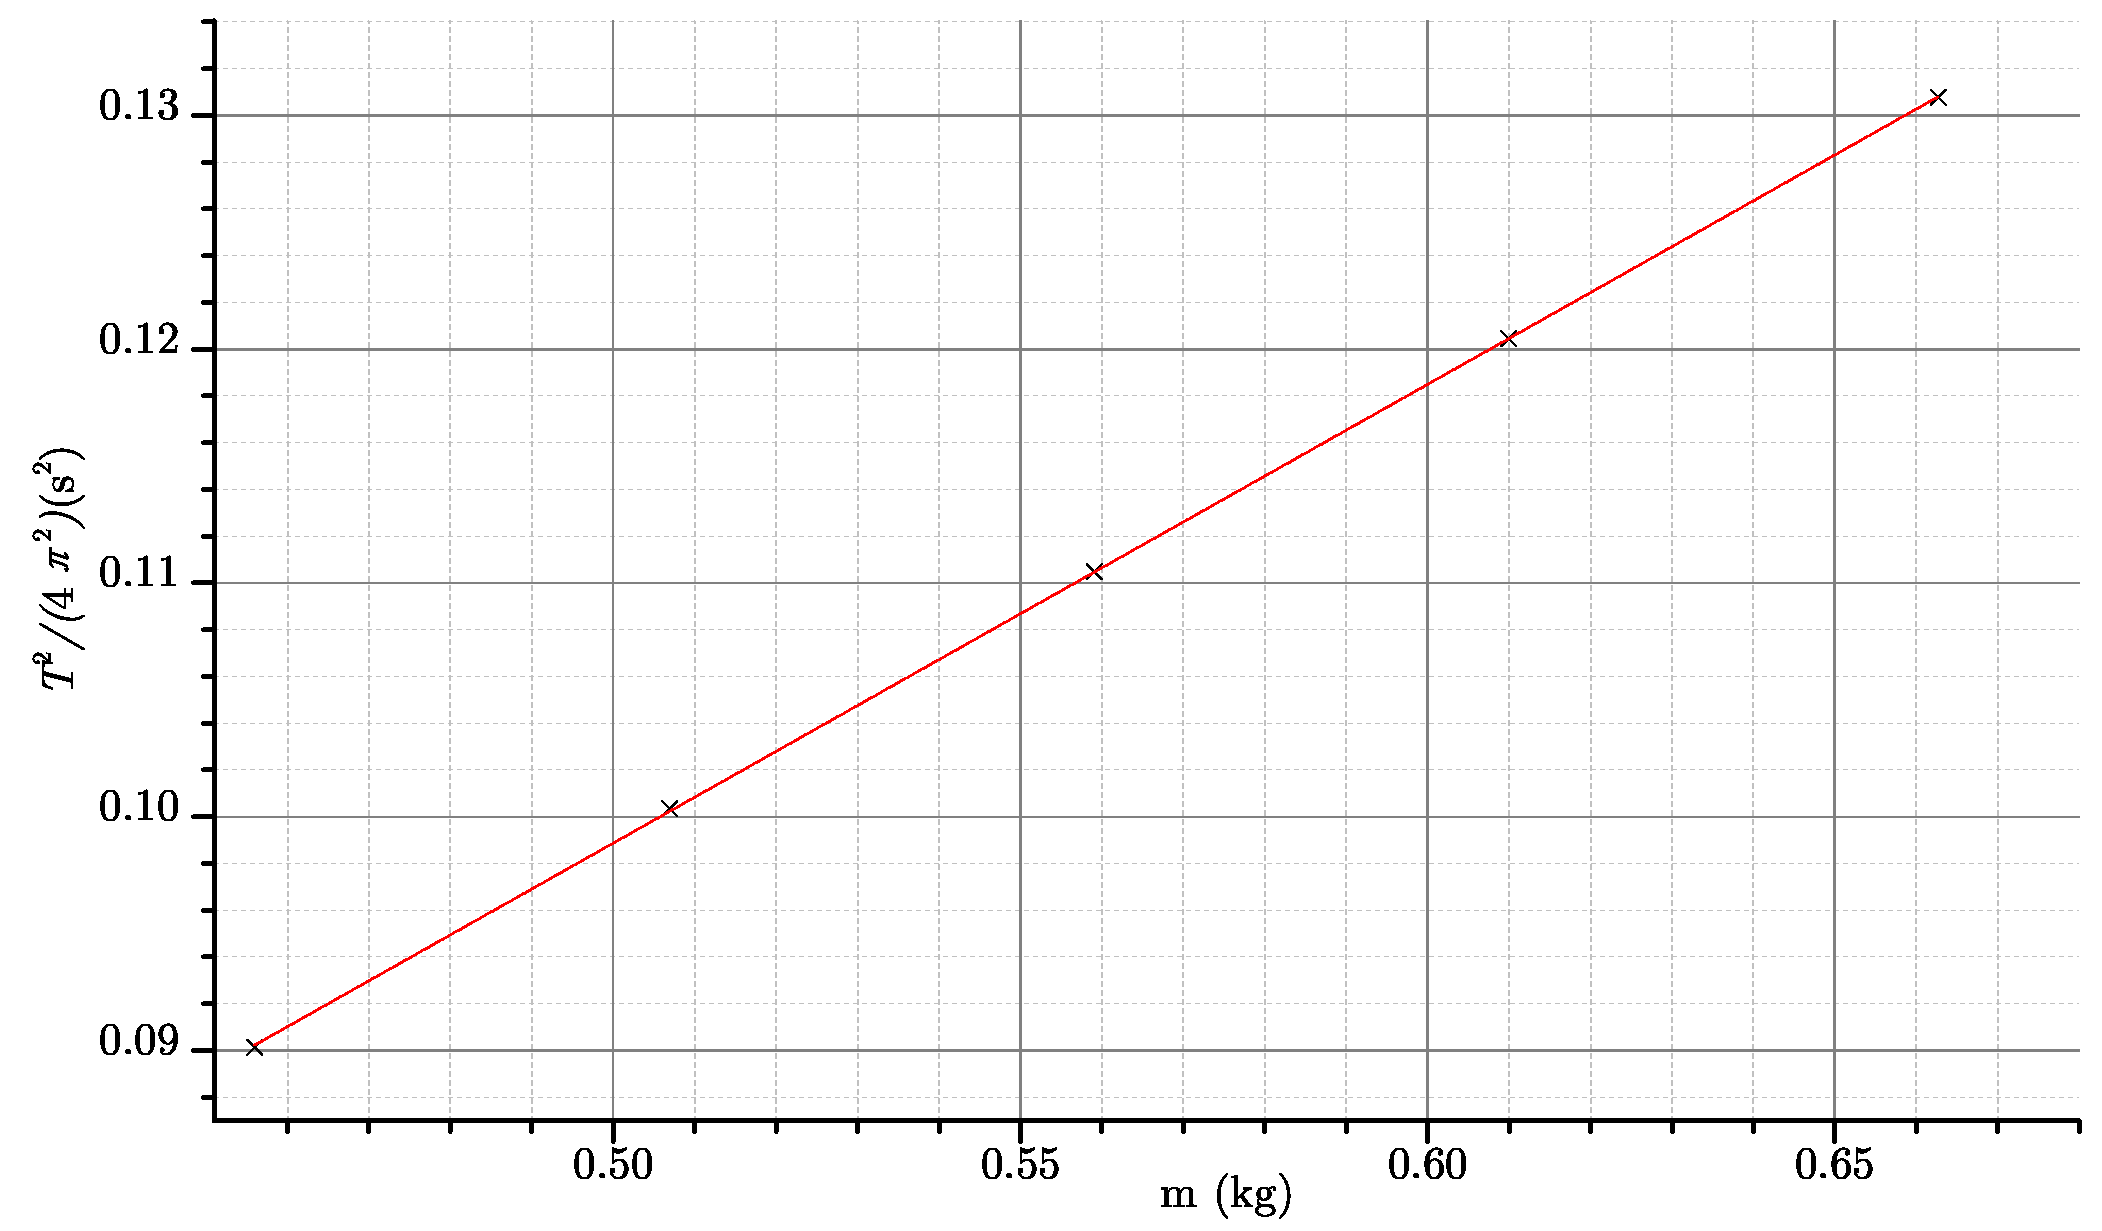
\includegraphics[width=\linewidth]{T-m.eps}
\end{center}
\paragraph{测量振子运动过程中的机械能}
这次我们研究振子在运动过程中速度随位置的变化,计算机械能$E=mv^2/2+kx^2/2$,分析它在运动过程中是否守恒。使用光电门计数器,配合一挡光片来测出振子在不同位置的速度。挡光宽度用游标卡尺测出,为$d=(\SI{1.492}{\cm}+\SI{.490}{\cm})/2=\SI{0.991}{\cm}$(测量U形片的外宽度与内宽度,其平均值即为挡光宽度。参见实验教材实验七习题第4题)。我们将振子拉到平衡位置相距\SI{40.0}{\cm}处释放,记录中间各位置的挡光时间,并计算出机械能,列于下表中。左右各自释放了三次,挡光时间取三次的平均值。注意无论从左还是从右释放,位置的记录都是按照以\SI{-40.0}{\cm}为起点,以运动方向为正方向的方式记录的。计算机械能时候所用的$k$为上一节所拟合出的$k$,$m$为\SI{456.00}{\g}加上弹簧质量的修正$m_0$之和。\SI{-40.0}{\cm}处按速度为零直接按弹簧势能给出机械能。
\begin{center}\begin{tabu} to \linewidth {X[c]|X[c]X[c]X[c]|X[c]X[c]||X[c]X[c]X[c]|X[c]X[c]}
\hline
$x/\si{cm}$	&$t$/s 左1 	&2	&3	&$\bar{t}/s$	&$E/J$&$t$/s 右1	&2	&3	&$\bar{t}/s$	&$E/J$
\\
\hline
(-40.0)	&	&	&	&	&0.4024	&&&&	&0.4024\\
-35.0	&0.01559	&0.01578	&0.01586	&0.01574	&0.4027	&0.01658	&0.01633	&0.01600	&0.01630	&0.3965\\
-28.0	&0.01071	&0.01069	&0.01072	&0.01071	&0.3942	&0.01062	&0.01068	&0.01065	&0.01065	&0.3962\\
-20.0	&0.00873	&0.00875	&0.00872	&0.00873	&0.3966	&0.00874	&0.00877	&0.00875	&0.00875	&0.3952\\
0.0	&0.00755	&0.00756	&0.00759	&0.00757	&0.3943	&0.00756	&0.00755	&0.00758	&0.00756	&0.3947\\
20.0	&0.00881	&0.00885	&0.00882	&0.00883	&0.3904	&0.00881	&0.00886	&0.00886	&0.00884	&0.3893\\
28.0	&0.01083	&0.01083	&0.01078	&0.01081	&0.3902	&0.01102	&0.01099	&0.01089	&0.01097	&0.3849\\
35.0	&0.01695	&0.01679	&0.01699	&0.01691	&0.3871	&0.01633	&0.01617	&0.01645	&0.01632	&0.3829\\
\hline
\end{tabu}\end{center}
可以看出,在实验误差范围内(从表中可以看出挡光时间的测量有\num{e-2}量级的随机误差),振子运动的机械能是近似守恒的,但总体上也存在着缓慢耗损的趋势。在从\SI{-40.0}{\cm}到\SI{35.0}{\cm}的运动过程中机械能大约损耗了约百分之五。这也与之前观察到的周期会随振幅增加而增加一个小量的现象相互印证,证明系统中存在着可被测到的阻尼。

\end{document} 